Na základě provedené analýzy máme nyní možnost připravit návrh řešení aplikace, která by zajistila správu modulárních dokumentů, jejich generování/publikaci.
Nesmíme zapomenout na důležité funkcionality. Jedná se hlavně o správu uživatelů, možnost tvořit revize a celkově verzovat jednotlivé části textu.
Dále nesmíme zapomenout na možnost rozšíření aplikace.

\section{Užitelská sekce}

V uživatelské sekci bude hlavní důraz kladen na správu uživatelů, zde také musíme myslet na ochranu jejich osobních udajů a díky GDPR také na
možnost jejich anonymizace. Také je potřeba brát v úvahu rozdělení uživatelů na standardní a administrátorské role, které mají rozdílné oprávnění.
Uživatelem se stává osoba při první interakci s aplikací, v tuto chvíli je osoba brána pouze jako host. Aby se uživatel stal plnohodnotným uživatelem,
je třeba se nejdříve registrovat, tím si uživatel vytvoří vlastní uživatelský účet, který bude mít standardní práva. Pro získání administrátorských
oprávnění je potřeba jiného administrátora, který může běžný účet prohlásit za administrátorský. Ještě bude existovat uživatel se oprávněním
\uv{super admin}, který bude mít práva na všechny operace v rámci systému.

V rámci zjednodušení práce s právy na jednotlivých dokumentech a repozitářích, o kterých se zmíníme později v této kapitole, zavedeme uživatelsky
definované role, které bude poté možné přiřazovat všem uživatelům. Tyto role budou sloužit k hromadným operacím na uživateli, toto ovšem bude
přístupné pouze uživatelům, kteří budou mít roli administrátora.

\subsection{GDPR}

Neboť bude naše aplikace pracovat s osobními údaji, je nutné toto brát na vědomí, proto se nyní podívejme na to, co musí naše aplikace splňovat, aby dodržela všechny
zákony o ochraně osobních údají a směrnice Evropské unie, GDPR. První co je nutné brát na vědomí je účel, za kterým údaje chceme údaje sbírat a uchovávat a jestli je náš
účel oprávněný. V tomto případě o uživateli získáme osobní údaj v podobě emailu, který stačí k identifikaci určité osoby. V našem případě je email identifikátor uživatele
a budeme jej při registraci žádat o souhlas se zpracováním osobních údajů. Dále musíme myslet na možnost smazání či anonymizace údajů uživatele. Toho docílíme ručními
zásahy do databáze, kde využijeme možnosti změnit email na jeho hash. \cite{gdpr}

\subsection{Příklady užití}

Nyní si připomeňme co naše aplikace musí určitě umět z uživatelské sekce, kdokoliv musí mít právo si založit svůj účet a mít možnost se do něho přihlásit.
Po přihlášení musí mít uživatel možnost změnit své vlastní údaje. Pro administrátorské účty musí být zpřístupněna možnost přiřadit role ostatním uživatelům
a zároveň ty role vytvářet, či mazat. Každý uživatel také musí disponovat možností deaktivovat svůj účet. Na obrázku \ref{fig:userFlow} je vidět, jak vypadá
cyklus přihlášení nebo registrace uživatele.

\section{Repozitáře}

Než začneme popisovat samotné generování dokumentů, je potřeba si definovat repozitáře našich modulů. Jednotlivé repozitáře nám budou sloužit jako složky,
které budou obsahovat moduly, ze kterých se pak budou skládat výsledné dokumenty. V rámci repozitářů je potřeba hlavně zajistit správně fungování oprávnění.
Pokud si uživatel založí nový repozitář, má vůči němu všechny práva, ostatní uživatelé se o tomto repozitáři v tomto stavu nemají jak dozvědět, je pro ně
skrytý. Pokud se ovšem zakladatel rozhodne svůj obsah repozitáře sdílet, má možnost sdílet repozitář s jednotlivými uživateli, uživatelskými rolemi a nebo
změnit repozitář na veřejný. Dále má také možnost definovat, jestli je repozitář pro jednotlivé uživatele pouze pro čtení, či použití modulu v dokumenty,
nebo jestli je možnost moduly i upravovat.

V neposlední řadě musíme myslet na verzování našich jednotlivých modulů, zde se nabízejí 2 možnosti jak tomuto přistoupit, buď by bylo možné integrovat
řešení založené na nějaké vcs (version control system), jedná se systém, který zařizuje verzování souborů,
nebo je možné implementovat verzování pomocí databáze. V této práci budeme volit verzování pomocí databáze a to hlavně z časových důvodů, neboť
pro použití vcs by bylo nutné udělat kompletní obal na nějaký již existující verzovací systém. Na digramu \ref{fig:moduleDia} je vidět jak by měly
vypadat vztahy mezi jednotlivými moduly.

\subsection{Přehled všech příkladů užití}

V repozitářích máme 2 hlavní části na které se musíme zaměřit, tou první je nutnost hlídat oprávnění a také je mít možnost spravovat. Tudíž majitel
repozitáře musí mít možnost ovlivňovat, kdo má, či nemá, přístup do jeho repozitáře. Dále musí mít možnost prohlásit svůj repozitář za veřejný a tím
dát možnost všem uživatelům do něj vstoupit. Krom oprávnění je potřeba také zajistit vytváření nových modulů a verzování jejich úprav. U verzování je
potřeba si pamatovat kdo a kdy vytvořil novou verzi. A také možnost vrátit se k určité předchozí verzi.

\section{Dokumenty}

Jelikož už máme definované chování pro jednotlivé repozitáře a jejich moduly, můžeme se vrhnout na návrh dokumentů, které se budou skládat z modulů. Každý
dokument je tedy soubor modulů, který je možné převést do tisknutelné podoby. Na co ale nesmíme zapomenout, že stejně jako moduly bude možné dokumenty také
verzovat, zde to bude provedeno pomocí revizí. Každá revize bude nést informace o tom, kdo danou revizi vytvořil a také ponese všechny informace o verzích
modulu, které jsou na danou revizi použity.

Podobně jako u repozitářů i u dokumentů budeme řešit oprávnění a to stejným způsobem, tudíž každý dokument má svého zakladatele nebo také vlastníka,
vlastník má možnost rozhodovat o tom, kdo bude moci dokument upravovat (vytvářet nové revize, měnit obsah dokumentu), a kdo bude mít možnost si pouze dokument
přečíst. Dále také bude možnost prohlásit dokument za veřejný a bude tedy přístupný všem uživatelům.

\subsection{Příklady užití v dokumentech}

Pro dokumenty bude důležité hlavně možnost jejich generovaní do přenosného formátu, jakým je například PDF. Dalším důležitou funkcionalitou bude možnost přiřazování
oprávnění jako je tomu u repozitářů, nesmí chybět ani možnost dokument prohlásit za veřejný a tím jej spřístupnit všem uživatelům. Je také potřeba myslet na možnost
procházet a generovat i starší revize.

\begin{figure}[h]
    \centering
    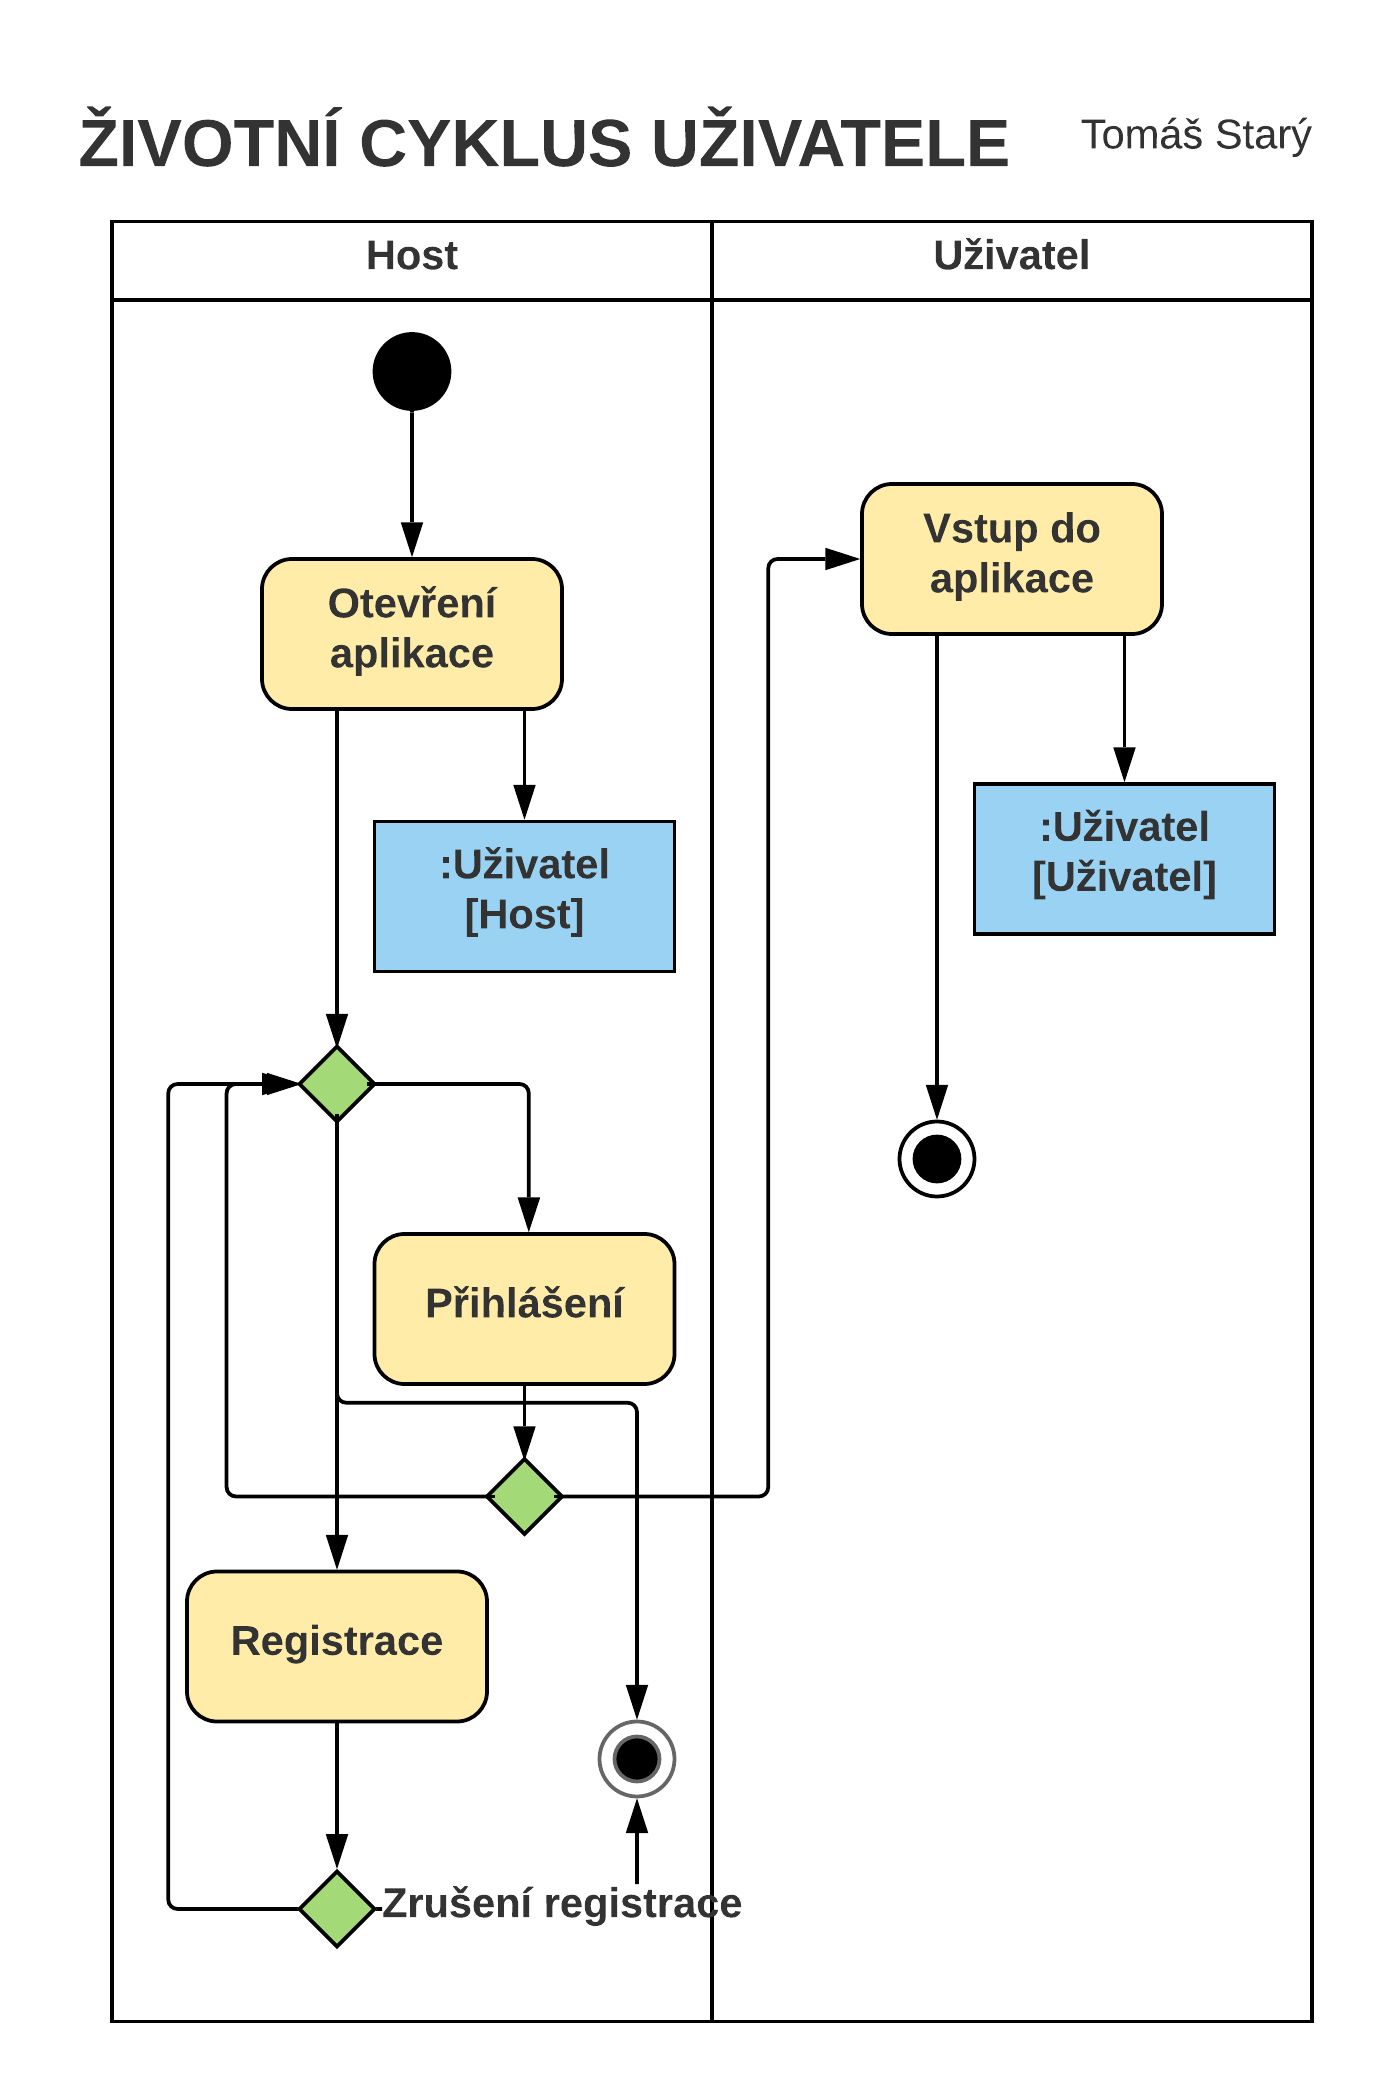
\includegraphics[width=\textwidth]{lifecycle.png}
    \caption{Diagram přihlášení a registrace uživatele}
    \label{fig:userFlow}
\end{figure}

\begin{figure}[h]
    \centering
    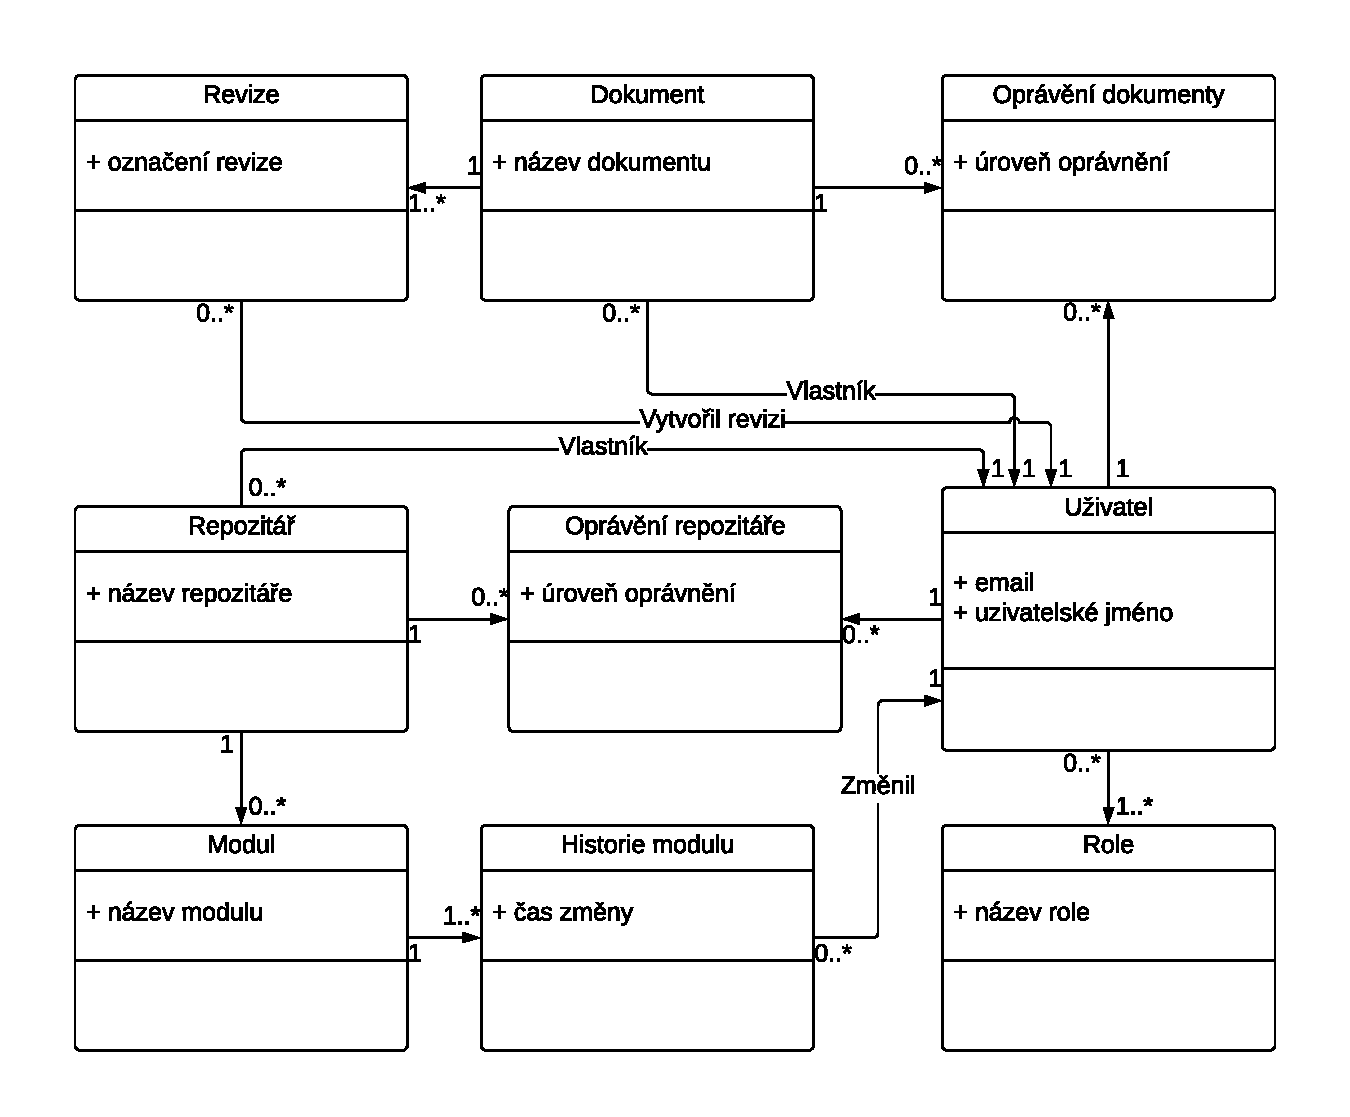
\includegraphics[width=\textwidth]{module_diagram.pdf}
    \caption{Návrh rozložení modelů}
    \label{fig:moduleDia}
\end{figure}